\chapter{Implementácia}
	V tejto kapitole sa pozrieme, s akými technológiami sme sa rozhodli pracovať a popíšeme najhlavnejšie časti zdrojového kódu. Ukážeme, čo spravíme pri registrácii nového používateľa, daľej čo pri nahrávaní súborov a na záver predvedieme, ako funguje sťahovanie a zdieľanie.
	
\section{Použité technológie}
	Zhrnieme si, aké technológie naša implementácia využíva na strane klienta, aké na strane servera a v krátkosti si ich popíšeme.
	\subsection{Back-end}
		Pod pojmom back-end máme na mysli implementáciu riešenia mimo používateľovho počítača. Na implementáciu serverovej časti sme sa rozhodli použiť Node.js s frameworkom Express, databázový systém MongoDB s pomocou objektového modelovacieho nástroju mongoose.
		\\
		\subsubsection{Node.js}
			Je platforma postavená na googlovskom V8 javascript engine, ktorý je napísaný v C++. Písať v jednom jazyku front-end aj back-end už dnes vďaka Node.js nie je problém. Celý model tejto platformy je postavený na udalostiach a neblokujúcich operáciách, takže je vhodný pre real-timeové aplikácie.
		\subsubsection{Express}
			Express je webový framework postavený na Node.js, ktorý nám zjednodušuje implementáciu backendu. S pomocou Expressu vieme veľmi ľahko vytvoriť REST API. Napísať čo sa stane, keď používateľ pristúpi pomocou metódy GET k webovej adrese \url{http://mojserver.sk/pes}, by mohlo vyzerať nasledovne:
			\medskip
			\begin{lstlisting}[caption=Express routing]
				app.get('/pes', function (req, res) {
					// nieco sa stane so psom, napriklad sa zobrazi na stranke
				});			
			\end{lstlisting}
		\subsubsection{MongoDB}
			MongoDB sme sa rozhodli použiť kvôli dynamickej schéme, škálovateľnosti, ale aj kvôli možnosti pracovať s moongose. Moongose je nástroj, ktorý nám dáva možnosť pracovať s databázou ako s obyčajnými objektami, čo výrazne urýchľuje vývoj. Pre ilustráciu, vytvorenie nového dokumentu v databáze bude vyzerať nasledovne:
			\medskip
			\begin{lstlisting}[caption=Vytvorenie mongoose modelu a jeho použitie]
				var Cat = mongoose.model('Cat', { name: String }); 

				var kitty = new Cat({ name: 'Murko' });
				kitty.save(function (err) {
 					if (err) // napriklad chyba v databaze
						console.log('mnau');
				});			
			\end{lstlisting}
			
		
	\subsection{Front-end}
		Za front-end budeme považovať všetky programy a scripty, ktoré sa dostanú k užívateľovi a budú zobrazované alebo vykonávané v jeho prehliadači. 
		\subsubsection{jQuery}
			Vačšina moderných prehliadačov vnútorne používa nejakú reprezentáciu na vykreslenie HTML, ktorú budeme nazývať objektový model dokumentu, tzv. DOM, z anglického Document Object Model. Pre prácu s DOM, používame knižnicu jQuery. Jej dokumentácia a developerská podpora je veľmi rozsiahla, čo uľahčuje jej používanie. 
			
		Knižnicu jQuery budeme tiež využívať na AJAX volania, pre ktoré nám poskytuje jednoduché API. AJAX slúži na výmenu dát medzi serverom a klientom bez nutnosti obnovovať stránku. Napríklad, keď si chceme vypýtať od servera privátny kľúč, pošleme požiadavku GET na adresu \url{http://server.com/getPrivKey} a dostaneme od neho odpoveď s privátnym kľúčom používateľa.
		\subsubsection{SJCL}
		Kryptografiu nám bude zaobstarávať knižnica Stanford Javascript Crypto Library, ktorej zdrojový kód a dokumentácia je online \cite{SJCLgit}. Táto open-source knižnica ponúka jednoduché rozhranie, pomocou ktorého vieme šifrovať a dešifrovať dáta. Podporuje symetrickú, aj asymetrickú kryptografiu, rôzne hašovacie funkcie a tiež umožňuje vytvárať a overovať podpisy. Okrem toho, že nám poskytuje všetky kryptografické primitíva, ktoré naše riešenie vyžaduje, jej hlavnou výhodou je efektívna implementácia. V rýchlosti šifrovania je v priemere štyrikrát rýchlejšia ako iné \cite{SJCLtext}. Kompatibilita medzi všetkými modernými prehliadačmi ako Chrome, Firefox, Safari a Internet Explorer v kombinácii s rýchlosťou a jednoduchým používateľským rozhraním boli kritickými prvkami pri výbere.



\section{Implementáciu návrhu}
	Túto časť venujeme prevažne zdrojovému kódu nášho riešenia. Uvedieme a vysvetlíme zdrojový kód registrácie, nahrávania a sťahovania dát a nakoniec sa pozrieme, ako funguje zdieľanie. Niektoré časti kódu pre jednoduchosť vynecháme a pokúsime sa uviesť iba tie najdôležitejšie časti. 
	
	\subsection{Registrácia}
	
		Aby sme vedeli s kým komunikujeme, potrebujeme najprv overiť jeho identitu. Na to sme sa rozhodli použiť protokol oAuth. S jeho pomocou dostaneme informácie o tom, s kým komunikujeme a zároveň používateľa autorizujeme k používaniu jeho GoogleDrive účtu. Následne potrebujeme vygenerovať privátny a verejný kľúč, vypýtať si od používateľa jeho univerzálne heslo a zašifrovať privátny kľúč univerzálnym heslom. Potom ho už len stačí poslať na server, kde sa uloží. 
		
		
\medskip
\begin{lstlisting}[caption=Generovanie kľúčového páru a odoslanie na server]
function generateKeyPair(callback) {
    var keys = sjcl.ecc.elGamal.generateKeys(256);

    //SERIALIZING KEYPAIR
    var pub = keys.pub.get();
    var sec = keys.sec.get();
    var serializedKeyPair = {
        pub: sjcl.codec.base64.fromBits(pub.x.concat(pub.y)),
        priv: sjcl.codec.base64.fromBits(sec)
    };

    // ASKING USER FOR HIS PASSWORD
    var passwd = prompt('Enter your new universal password.  You will need this password to decrypt and share files', 'Password here');
    // ENCRYPTING USERS PRIVATE KEY
    var enc = sjcl.encrypt(passwd, serializedKeyPair.priv);
    serializedKeyPair.priv = enc;

    // SENDING KEYPAIR TO SERVER
    saveKeyPair(serializedKeyPair, callback);
}

function saveKeyPair(keyPair, callback) {
    // SEND KEYPAIR TO SERVER
    $.post('/saveKeypair', keyPair, function (res2) {
        callback(res2);
    });
}
\end{lstlisting}


	\subsection{Nahrávanie dát}	
	
		Keď chceme uložiť ľubovolné dáta v cloude v šifrovanej forme, najprv potrebujeme načítať súbor.
\medskip
\begin{lstlisting}[caption=Načítanie súboru]		
function uploadFile() {
    if ($('input#uplFile')[0].files[0] != undefined){
        updateFileResumableGoogle({'title': $('input#uplFile')[0].files[0].name + '.sc'}, $('input#uplFile')[0].files[0], function (uplResp) {// possible to add callback});
    }
}
\end{lstlisting}		

		Po načítaní celého súboru vygenerujeme náhodný kľúč, ktorý použijeme na zašifrovanie dát súboru. Zo servera si vypýtame náš verejný kľúč a ním zašifrujeme kľúč použitý na šifrovanie súboru. Nakoniec odošleme súbor do cloudu a zašifrované súborové heslo na server. \\
		Väčšina našich funkcií používa tzv. callback, čo je funkcia, ktorá sa zavolá po skončení predchádzajúcej funkcie. Napríklad, keď zavoláme getPubKey(email, callback), najprv sa vykoná funkcia getPubKey, a keď skončí svoju prácu, zavolá funkciu callback(pubKey). Ako parameter je vždy návratová hodnota predchádzajúcej funkcie.
		
		
\medskip
\begin{lstlisting}[caption=Upload súboru, firstnumber=6]		
function updateFileResumableGoogle(metadata, fileData, callback) {
    var accessToken = gapi.auth.getToken().access_token;
    var email = $.cookie('email');

    //GET PUBLIC KEY OF LOGGED USER
    getPubKey(email, function(pubKey) {

        //GENERATE PASSWORD FOR FILE ENCRYPTION
        createRandomString(function (passString) {

            // FILE UPLOAD
            var reader = new FileReader();
            reader.readAsArrayBuffer(fileData);
            reader.onload = function() {
            
                //FILE ENCRYPTION
                var bits = sjcl.codec.bytes.toBits(new Uint8Array(reader.result));
                var crypt = sjcl.encrypt(passString, bits);
                var blob = new Blob([crypt]);

                //ACTUAL UPLOADING
                var uploader = new MediaUploader({
                    metadata: metadata,
                    file: blob,
                    token: accessToken,
                    onComplete: function(gResp) {

                        //FILE PASSWORD ENCRYPTION
                        var encPass = sjcl.encrypt(pubKey, passString);
                        gResp = JSON.parse(gResp);

                        //SENDING ENCRYPTED FILE PASSWORD TO SERVER
                        saveFileKey(email, encPass, gResp.id, callback);
                    },
                    onError: function(err) {
                        log(err);
                    }
                });
                uploader.upload();
            };
        });
    });
}
\end{lstlisting}		
	
		\begin{figure}[H]
			\begin{center}
				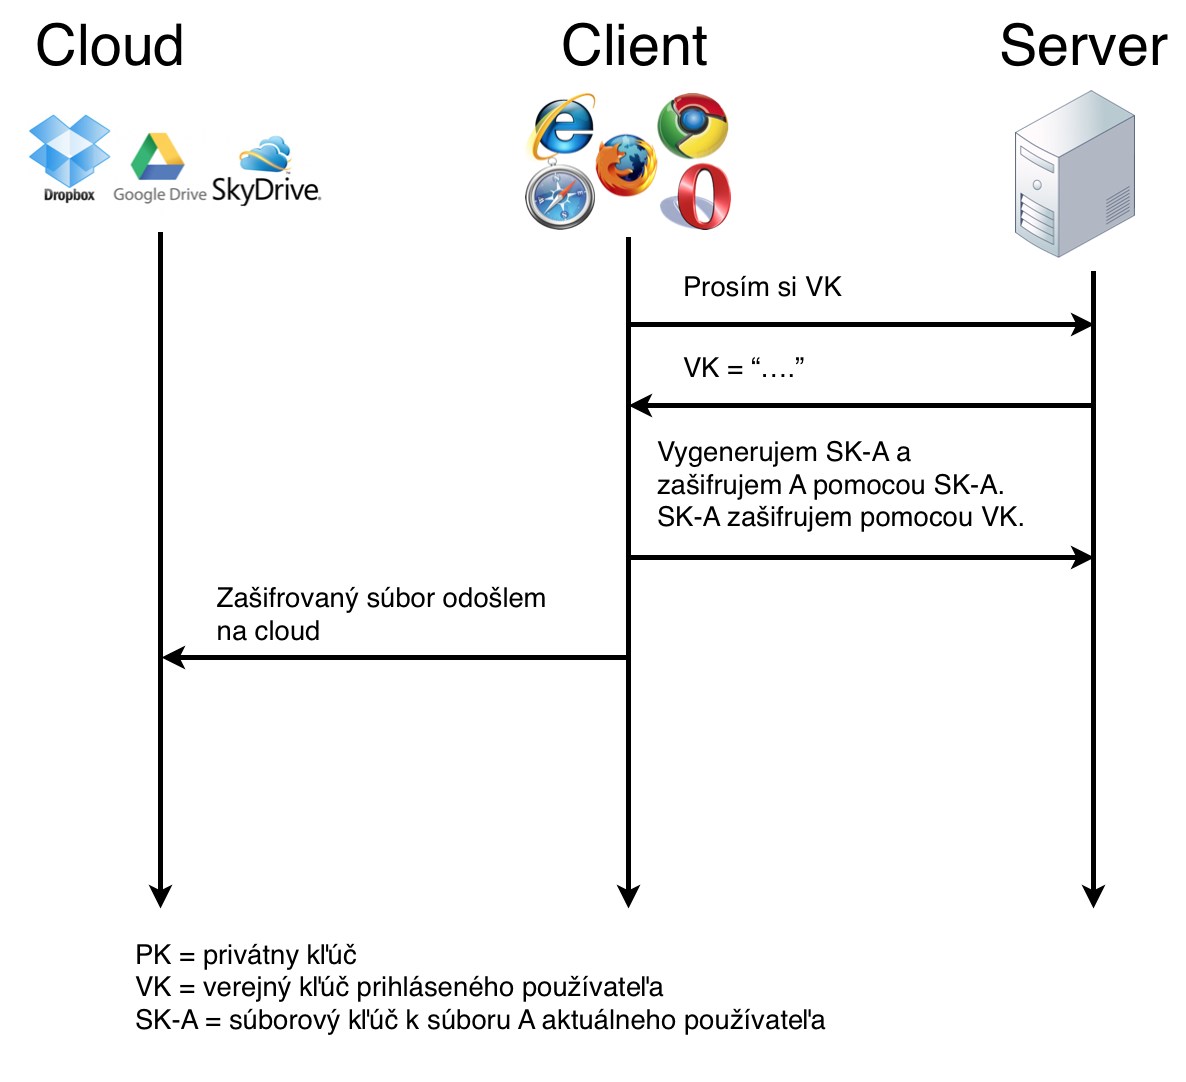
\includegraphics[width=1\linewidth]{images/nahravanie_com.png}
				\caption{Komunikácia pri nahrávaní súboru na server}
			\end{center}
		\end{figure}
	
	\subsection{Sťahovanie dát}
	
		V prípade sťahovania súborov si klikneme na súbor vo webovom rozhraní a potom na tlačítko "Download", ktoré vykoná niekoľko akcií. V prvom rade získame zo servera privátny kľúč a rozšifrujeme ho naším univerzálnym heslom.
		

		
\medskip
\begin{lstlisting}[caption=Získanie privátneho kľúča]	
function getPrivKey(callback) {
    $.get('/getPrivKey', function(res) {
        // DECRYPTS PRIVATE KEY WITH USERS KEY
        var userKey = prompt('Please enter your password', 'Enter your password here');
        var privKey = sjcl.decrypt(userKey, res);

        // DESERIALIZING PRIVATE KEY
        var sec = new sjcl.ecc.elGamal.secretKey(
            sjcl.ecc.curves.c256,
            sjcl.ecc.curves.c256.field.fromBits(sjcl.codec.base64.toBits(privKey))
        );

        callback(sec);
    });
}
\end{lstlisting}

		Keď ho už máme k dispozícii, požiadame server o zašifrovaný kľúč k súboru a rozšifrujeme ho pomocou privátneho kľúča.

\begin{lstlisting}[caption=Získanie súborového kľúča, firstnumber=16, ,label={getFileKeyLabel}]	
function getFileKey(fileId, callback) {
    getPrivKey(function (privKey) {
        $.post('/getFileKey', {'fileId': fileId}, function(encFileKey) {

            // DECRYPTS FILE KEY WITH USERS PRIVATE KEY
            var fileKey = sjcl.decrypt(privKey, encFileKey);

            callback(fileKey);
        });
    })
}
\end{lstlisting}

		Teraz už môžme prejsť k samotnému stiahnutiu súboru a jeho rozšifrovaniu. 
		
\begin{lstlisting}[caption=Stiahnutie súboru, firstnumber=27]	
function downloadFileGoogle(file, callback) {
    if (file.downloadUrl) {
        var accessToken = gapi.auth.getToken().access_token;
        var xhr = new XMLHttpRequest();
        xhr.open('GET', file.downloadUrl);
        xhr.setRequestHeader('Authorization', 'Bearer ' + accessToken);
        
        // ITS ENCRYPTED FILE
        xhr.onload = function() {
            getFileKey(file.id, function(fileKey) {

                // DECRYPT FILE
                var base64decrypt = sjcl.decrypt(fileKey, xhr.response, {'raw': 1});
                var byteArray = new Uint8Array(sjcl.codec.bytes.fromBits(base64decrypt));

                // PASS DOWNLOADED FILE TO CALLBACK
                callback({
                    'title': title,
                    'data': byteArray
                });
            });
        };
        xhr.onerror = function() {
            console.log("ERROR!");
        };
        xhr.send();
    } else {
        console.log("ERROR MISSING DOWNLOAD URL");
    }
}
\end{lstlisting}

		Keď všetko prebehne úspešne zavoláme callback funkciu, ktorej parametre budú meno súboru a jeho dáta. 
		
		\begin{figure}[H]
			\begin{center}
				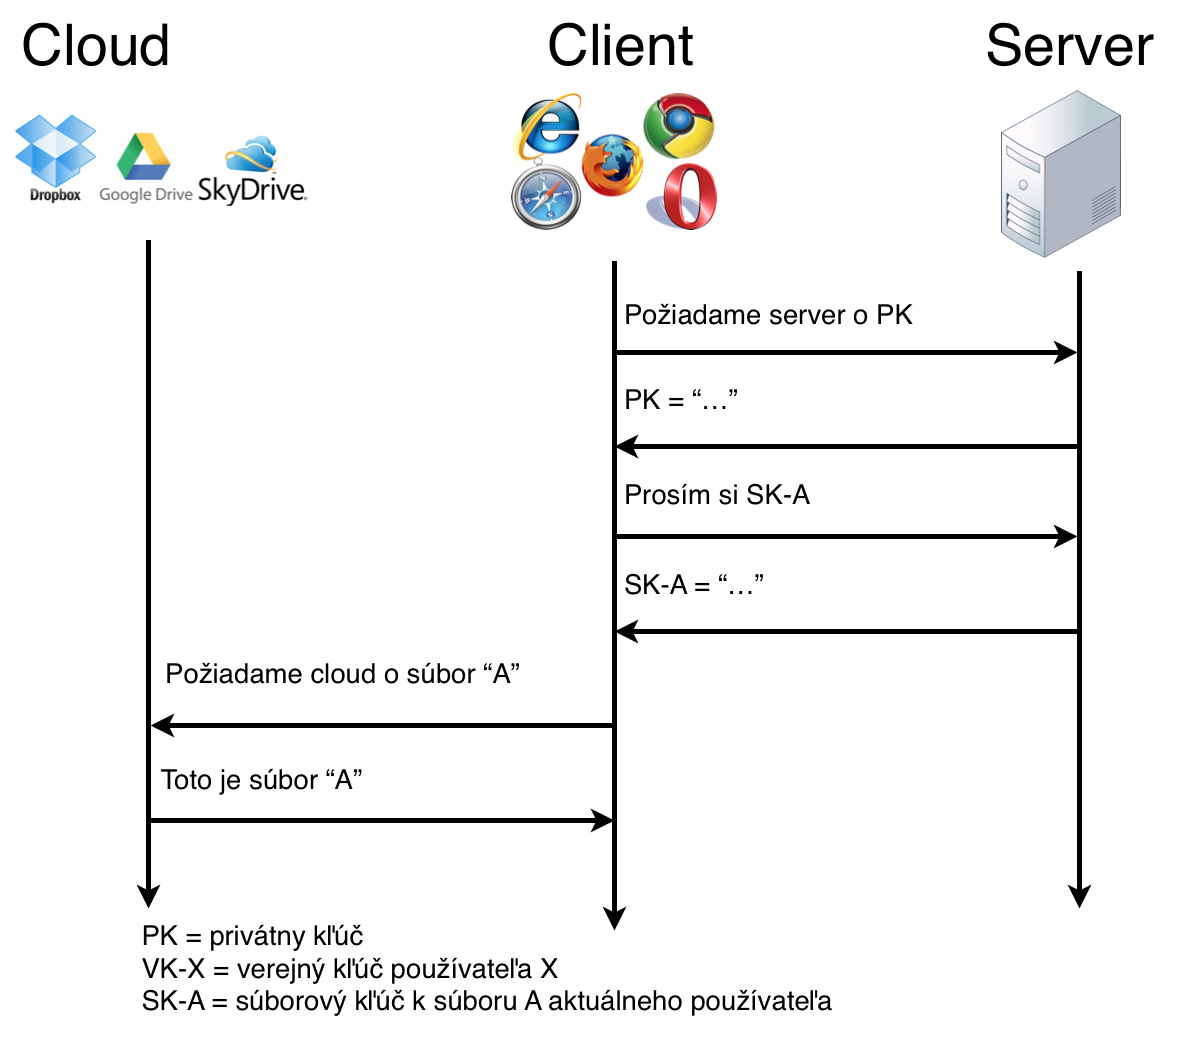
\includegraphics[width=1\linewidth]{images/stahovanie_com.png}
				\caption{Komunikácia pri sťahovaní súboru na server}
			\end{center}
		\end{figure}
	
	\subsection{Zdieľanie dát}
		
		To, čo robí naše riešenie zaujímavým, je zdieľanie súborov. Pre zdieľanie súboru nám stačí zavolať funkciu, ktorej dáme štyri parametre. ID súboru, email používateľa, s ktorým chceme zdieľať, rolu a funkciu, ktorá sa má po skončení funkcie vykonať. Parameter role nám hovorí, aké právomoci má používateľ k tomu súboru. Môže byť čitateľ, čo mu umožní súbor iba čítať, zapisovateľ, ktorý môže meniť dáta súboru, alebo vlastník, čo znamená, že môže robiť všetko ako čitateľ a zapisovateľ, ale naviac môže súbor aj zmazať. Celý proces zdieľania vyžaduje niekoľko krokov. V prvom rade musíme získať kľúč k súboru rovnako ako pri sťahovaní dát. Potom potrebujeme verejný kľúč používateľa, s ktorým plánujeme zdieľať súbor. Následne zašifrujeme súborový kľúč verejným kľúčom, ktorý sme získali a uložíme ho na server. A napokon už len stačí požiadať cloud, aby povolil prístup k súboru používateľovi, s ktorým sme sa rozhodli podeliť o naše dáta.
		

		
\begin{lstlisting}[caption=Zdieľanie súboru]	
function shareFileGoogle(fileId, email, role, callback) {

    getFileKey(fileId, function(fileKey) {
        getPubKey(email, function (pubKey) {

            //ENCRYPT FILEKEY WITH PUB-KEY OF USER I AM SHARING WITH
            var shareFileKey = sjcl.encrypt(pubKey, fileKey);

            //SAVE NEW ENCRYPTED KEY
            saveFileKey(email, shareFileKey, fileId, function(saveFileKeyResponse) {

                //SHARE ON GOOGLE DRIVE (ADD PERMISSION FOR USER)
                insertPermissionGoogle(fileId, email, 'user', role, function(resp) {
                    callback(resp);
                });
            });
        });
    });
}
\end{lstlisting}		
	
		\begin{figure}[H]
			\begin{center}
				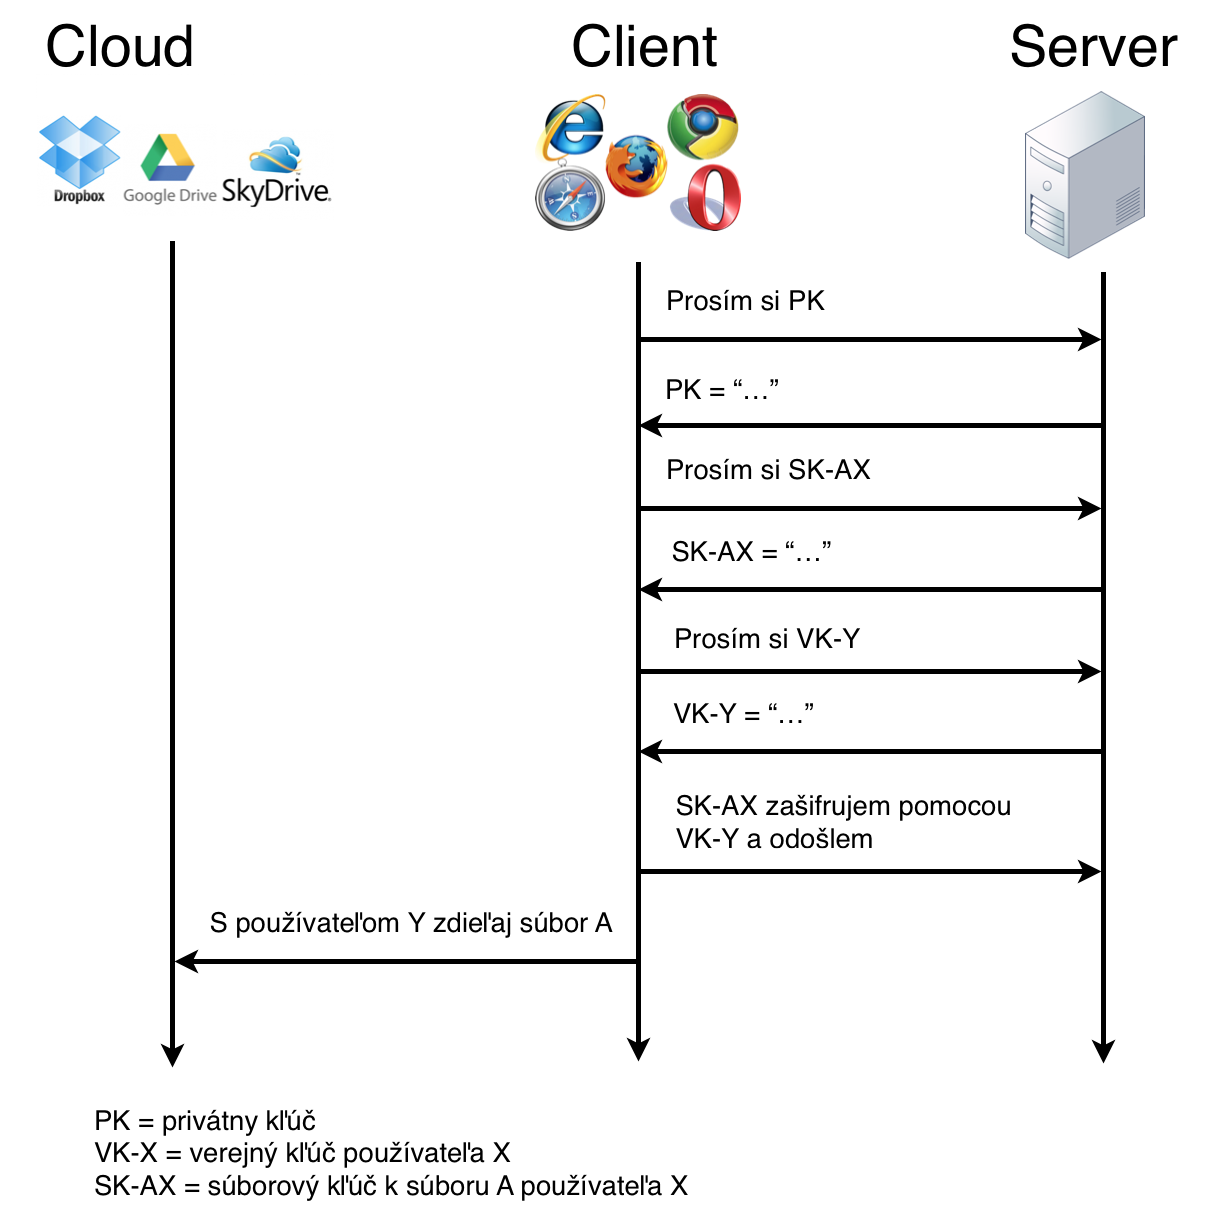
\includegraphics[width=1\linewidth]{images/zdielanie_com.png}
				\caption{Komunikácia pri zdieľaní súboru na server}
			\end{center}
		\end{figure}
	
	\subsection{Zrušenie zdieľania}
	
		Aby sme naše dáta prestali zdieľať, stačí požiadať cloud o zrušenie prístupu k súboru a aby sme zbytočne nezaplňovali databázu vymažeme aj súborový kľúč zo servera. 
	
\begin{lstlisting}[caption=Zrušenie zdieľania súboru]		
function stopShareingFileGoogle(fileId, email, callback) {
    retrievePermissions(fileId, function(permissions) {
        for(var permission in permissions) {
            if (permissions[permission].emailAddress == email) {
                var permId = permissions[permission].id;
                removePermissionGoogle(fileId, permId, function(resp) {
                    callback(resp);
                });
            }
        }
    });
}
\end{lstlisting}	